\documentclass[12pt, a4paper]{report}

\usepackage{uit-report}
\usepackage{url}
\urlstyle{tt}

% ============================================================
\begin{document}

% ==================== TRANG BÌA ====================
\pagenumbering{gobble}
% ==================== TRANG BÌA ====================
\begin{titlepage}
\thispagestyle{empty}
% Khung viền tikz chuẩn UIT
\begin{tikzpicture}[remember picture, overlay]
  \draw[line width=1pt, color=blue!80!black]
    ($(current page.north west) + (108pt,-65pt)$)
    rectangle
    ($(current page.south east) + (-56pt,56pt)$);
\end{tikzpicture}

\vspace*{0pt} % reset vertical position
\begin{center}
  {\large\bfseries ĐẠI HỌC QUỐC GIA THÀNH PHỐ HỒ CHÍ MINH}\\[3pt]
  {\large\bfseries TRƯỜNG ĐẠI HỌC CÔNG NGHỆ THÔNG TIN}\\[3pt]
  {\normalsize\bfseries KHOA MẠNG MÁY TÍNH VÀ TRUYỀN THÔNG}\\[24pt]

  % Logo UIT
  
\includegraphics[height=2.2cm]{img/logo/logo_uit.png}\\[14pt]

  {\large\bfseries BÁO CÁO ĐỒ ÁN CUỐI KỲ}\\[5pt]
  {\normalsize\bfseries MÔN HỌC: NT533 -- [TÊN MÔN HỌC CHƯA CUNG CẤP]}\\[18pt]

  {\normalsize\bfseries ĐỀ TÀI}\\[8pt]
  {\large\bfseries XÂY DỰNG HỆ THỐNG DISASTER RECOVERY ĐA VÙNG\\TỐI ƯU CHI PHÍ TRÊN AMAZON WEB SERVICES}\\[12pt]
  {\normalsize\bfseries DESIGN AND IMPLEMENTATION OF A COST-OPTIMIZED\\MULTI-REGION DISASTER RECOVERY SYSTEM ON AWS}\\[32pt]

  % Thông tin GVHD và nhóm SV — dùng minipage căn giữa
  \begin{minipage}{0.75\textwidth}
    \raggedright
    {\bfseries Lớp:}\enspace [MÃ LỚP HỌC PHẦN CHƯA CUNG CẤP]\\[10pt]
    {\bfseries Giảng viên hướng dẫn:}\\[4pt]
    \hspace{0.5cm}1.\enspace [GIẢNG VIÊN CHƯA CUNG CẤP]\\[10pt]
    {\bfseries Nhóm sinh viên thực hiện:}\\[4pt]
    \hspace{0.5cm}1.\enspace [HỌ TÊN SINH VIÊN CHƯA CUNG CẤP] \hfill [MSSV CHƯA CUNG CẤP]
  \end{minipage}

  \vfill
  {\bfseries TP. Hồ Chí Minh, tháng 10 năm 2026}
\end{center}
\end{titlepage}


% ==================== PHẦN ĐẦU (ROMAN) ====================
\pagenumbering{roman}
\pagestyle{empty}
\fancypagestyle{plain}{\fancyhf{}\renewcommand{\headrulewidth}{0pt}\renewcommand{\footrulewidth}{0pt}}

\chapter*{Lời cảm ơn}
%\markboth{LỜI CẢM ƠN}

Nhóm tác giả trân trọng cảm ơn giảng viên phụ trách môn học NT533 và Khoa Mạng máy tính và Truyền thông, Trường Đại học Công nghệ Thông tin, đã tạo điều kiện để nhóm nghiên cứu bài toán duy trì khả năng phục hồi của hệ thống trên nền tảng điện toán đám mây. Những kiến thức về kiến trúc AWS, tự động hóa hạ tầng và vận hành dịch vụ là cơ sở để nhóm xây dựng, triển khai và đánh giá mô hình Disaster Recovery đa vùng trong đồ án này.

Nhóm cũng cảm ơn các thành viên đã cùng phân tích yêu cầu, xây dựng mã nguồn, triển khai hạ tầng, thực hiện kiểm thử và hoàn thiện báo cáo. Kết quả đồ án là cơ hội để nhóm hiểu rõ hơn mối quan hệ giữa thiết kế kiến trúc, tự động hóa và hoạt động phục hồi trong môi trường cloud thực tế.


{
\begin{table}[ht]
\centering
\begin{tabular}{>{\centering}m{0.4\textwidth}>{\centering\arraybackslash}m{0.5\textwidth}}
 & \textbf{Nhóm tác giả}\\
 & [THÔNG TIN NHÓM CHƯA CUNG CẤP]
\end{tabular}
\end{table}
}

\clearpage
\chapter*{Tóm tắt}
%\markboth{TÓM TẮT}
Đồ án xây dựng hệ thống Disaster Recovery đa vùng trên Amazon Web Services theo chiến lược Backup and Restore nhằm cân bằng giữa khả năng phục hồi và chi phí duy trì Region dự phòng. Workload chính được triển khai tại Sydney (\texttt{ap-southeast-2}), gồm Amazon VPC, Application Load Balancer, ba dịch vụ Amazon ECS Fargate và Amazon RDS for PostgreSQL. Singapore (\texttt{ap-southeast-1}) lưu giữ recovery point của AWS Backup, bản sao image Amazon ECR, thông tin xác thực trong AWS Secrets Manager và control plane tự động hóa. Hạ tầng runtime tại vùng DR chỉ được tạo khi quy trình phục hồi được kích hoạt.

Hệ thống được mô hình hóa bằng các nested stack AWS CloudFormation. AWS Step Functions điều phối quá trình xác nhận sự cố, tạo hạ tầng runtime, khôi phục RDS, cập nhật secret, scale ECS và kiểm tra sức khỏe các target group. DynamoDB lock ngăn workflow chạy trùng; EventBridge và SNS hỗ trợ kích hoạt và thông báo. Chế độ safe test cho phép kiểm thử toàn bộ đường phục hồi mà không thay đổi Route~53 production.

Trong lần thực nghiệm ngày 30/09/2026, DR runtime được tạo thành công tại Singapore, AWS Backup restore RDS hoàn tất và ba ECS service đạt trạng thái healthy. Ứng dụng vượt ALB health gate sau khoảng 19 phút 15 giây kể từ lúc workflow bắt đầu; bước cuối ngay trước trạng thái thành công hoàn tất sau khoảng 19 phút 17 giây. Kết quả cho thấy mô hình có khả năng tự động hóa phần lớn quá trình phục hồi mà không cần duy trì compute và database thường trực tại Region thứ hai. Những hướng phát triển chính gồm tự động lưu evidence, kiểm thử lặp lại, xây dựng failback và tăng tính sẵn sàng trong từng Region.

\vspace{0.5em}
\noindent\textbf{Từ khóa:} Disaster Recovery, Multi-Region, AWS Backup, Amazon ECS Fargate, Amazon RDS, AWS Step Functions, Infrastructure as Code.

\chapter*{Abstract}
This project implements a cost-optimized multi-region disaster recovery system on Amazon Web Services using the Backup and Restore strategy. The primary workload runs in Sydney, while Singapore retains cross-region backups, replicated container images, replicated credentials, and the recovery control plane. AWS Step Functions orchestrates on-demand infrastructure provisioning, RDS restoration, secret updates, ECS scaling, and Application Load Balancer health validation. A safe recovery exercise performed on September 30, 2026 provisioned the Singapore runtime and restored the application without changing production DNS. The application passed the ALB health gate approximately 19 minutes 15 seconds after the workflow started, and the final workflow step completed after approximately 19 minutes 17 seconds. The result demonstrates that the design can automate the main recovery path while avoiding continuously running compute and database resources in the secondary Region.

\clearpage

% Mục lục (không đánh số trang)
\tableofcontents
\clearpage
\pagestyle{customfancy}
\fancypagestyle{plain}{\fancyhf{}\fancyfoot[C]{\thepage}\renewcommand{\headrulewidth}{0pt}\renewcommand{\footrulewidth}{0pt}}

% Danh mục hình ảnh
\begingroup
\renewcommand*{\addvspace}[1]{}
\phantomsection
\addcontentsline{toc}{chapter}{DANH MỤC HÌNH ẢNH}
\listoffigures
\clearpage

% Danh mục bảng biểu
\phantomsection
\addcontentsline{toc}{chapter}{DANH MỤC BẢNG BIỂU}
\listoftables
\clearpage

% Danh mục từ viết tắt
\chapter*{DANH MỤC TỪ VIẾT TẮT}
\addcontentsline{toc}{chapter}{DANH MỤC TỪ VIẾT TẮT}

\begin{table}[h]
    \centering
    \begin{tabularx}{\textwidth}{l X}
    \toprule
    \textbf{Chữ viết tắt} & \textbf{Chữ viết đầy đủ} \\
    \midrule
    ALB & Application Load Balancer \\
    API & Application Programming Interface \\
    AWS & Amazon Web Services \\
    AZ & Availability Zone \\
    CI/CD & Continuous Integration / Continuous Delivery \\
    DR & Disaster Recovery \\
    ECR & Elastic Container Registry \\
    ECS & Elastic Container Service \\
    IAM & Identity and Access Management \\
    IaC & Infrastructure as Code \\
    KMS & Key Management Service \\
    NAT & Network Address Translation \\
    RDS & Relational Database Service \\
    RPO & Recovery Point Objective \\
    RTO & Recovery Time Objective \\
    SG & Security Group \\
    SNS & Simple Notification Service \\
    TTL & Time to Live \\
    UIT & University of Information Technology \\
    VPC & Virtual Private Cloud \\
    \bottomrule
    \end{tabularx}
\end{table}

\clearpage

% Danh mục mã nguồn
\phantomsection
\addcontentsline{toc}{chapter}{DANH MỤC MÃ NGUỒN}
\lstlistoflistings
\clearpage
\endgroup

% ==================== NỘI DUNG CHÍNH (ARABIC) ====================
\pagenumbering{arabic}
\setcounter{page}{1}

\chapter{TỔNG QUAN ĐỀ TÀI}
\label{c:tongquan}
\section{Bối cảnh và động lực}

Điện toán đám mây giúp tổ chức triển khai ứng dụng nhanh, mở rộng theo nhu cầu và giảm chi phí đầu tư hạ tầng ban đầu. Tuy nhiên, việc đưa workload lên cloud không tự động loại bỏ rủi ro gián đoạn. Lỗi phần mềm, sai cấu hình, mất dữ liệu, sự cố mạng hoặc sự cố ở phạm vi Availability Zone và Region vẫn có thể làm dịch vụ ngừng hoạt động. AWS Well-Architected Reliability Pillar xem khôi phục sau thảm họa là một phần của thiết kế độ tin cậy và yêu cầu quy trình phục hồi phải được chuẩn bị, kiểm thử định kỳ \cite{aws-dr-objectives}.

Đối với hệ thống quy mô vừa và nhỏ, duy trì đầy đủ ứng dụng và cơ sở dữ liệu tại hai Region tạo ra chi phí thường trực đáng kể. Ngược lại, phương án chỉ lưu bản sao dữ liệu giúp giảm chi phí chờ nhưng cần nhiều thời gian hơn để dựng lại hạ tầng khi có sự cố. Đồ án tập trung giải quyết điểm đánh đổi này bằng chiến lược Backup and Restore: các artifact cần thiết được chuẩn bị tại Region dự phòng, còn compute và database chỉ được khởi tạo khi quy trình DR bắt đầu.

\section{Bài toán của đề tài}

Hệ thống được triển khai với workload chính tại Sydney và Region dự phòng tại Singapore. Khi Primary Region không còn đáp ứng, quy trình phục hồi cần thực hiện đồng bộ nhiều công việc:

\begin{enumerate}
  \item lựa chọn recovery point PostgreSQL đã được sao chép sang Singapore;
  \item tạo mạng, load balancer và ECS runtime tại Region dự phòng;
  \item khôi phục RDS, cập nhật thông tin kết nối và khởi chạy ứng dụng;
  \item kiểm tra sức khỏe của toàn bộ target group trước khi cho phép chuyển lưu lượng;
  \item ngăn nhiều quy trình DR chạy đồng thời và hỗ trợ cleanup an toàn sau kiểm thử.
\end{enumerate}

Một bản backup riêng lẻ chưa đủ tạo thành dịch vụ có thể tiếp nhận request. Quá trình phục hồi còn phụ thuộc vào network, IAM, container image, secret, database endpoint, health check và thứ tự khởi tạo tài nguyên. Vì vậy, hệ thống được thiết kế như một workflow có trạng thái thay vì một tập hợp lệnh vận hành rời rạc.

\section{Mục tiêu}

Mục tiêu tổng quát của đồ án là xây dựng hệ thống Disaster Recovery đa vùng trên AWS theo chiến lược Backup and Restore, có khả năng tái tạo workload tại Singapore từ các artifact đã chuẩn bị trước. Các mục tiêu cụ thể gồm:

\begin{itemize}
  \item mô tả hạ tầng bằng AWS CloudFormation để có thể triển khai lặp lại;
  \item container hóa ứng dụng và vận hành trên Amazon ECS Fargate;
  \item lưu dữ liệu trên Amazon RDS for PostgreSQL và sao chép recovery point liên vùng bằng AWS Backup;
  \item sao chép image ECR và thông tin xác thực cần thiết sang Region dự phòng;
  \item điều phối quy trình phục hồi bằng AWS Step Functions với retry, timeout, lock và health gate;
  \item cung cấp chế độ kiểm thử an toàn, không mặc định thay đổi DNS production;
  \item thu thập các mốc thời gian thực tế để đánh giá quá trình phục hồi.
\end{itemize}

\section{Phạm vi}

Đề tài tập trung vào việc xây dựng và tự động hóa quy trình khôi phục workload từ Primary Region sang DR Region. Phạm vi triển khai gồm hạ tầng mạng, Application Load Balancer, ba dịch vụ ECS Fargate, RDS PostgreSQL, backup liên vùng, container image, secret và hệ thống điều phối phục hồi.

Primary Region đặt tại Sydney (\texttt{ap-southeast-2}); DR Region đặt tại Singapore (\texttt{ap-southeast-1}). Ứng dụng demo sử dụng chung một image cho ba service \texttt{auth}, \texttt{product} và \texttt{order}. Service product cung cấp các thao tác dữ liệu tối thiểu trên PostgreSQL; hai service còn lại hỗ trợ minh họa định tuyến và kiểm tra khả năng khởi chạy nhiều workload.

Đồ án lựa chọn Backup and Restore thay vì Active/Active hoặc Warm Standby nhằm ưu tiên chi phí duy trì thấp. Các nội dung đánh giá tải lớn, failback tự động và kiến trúc ứng dụng production hoàn chỉnh được xem là hướng mở rộng sau khi quy trình DR cốt lõi đã hoạt động ổn định.

\section{Phương pháp thực hiện}

Nhóm triển khai hệ thống theo bốn bước. Trước hết, kiến trúc đa vùng được mô hình hóa bằng các nested stack CloudFormation. Tiếp theo, ứng dụng và các artifact được chuẩn bị tại Sydney và sao chép sang Singapore. Sau đó, Step Functions được xây dựng để điều phối toàn bộ quy trình tạo runtime, restore RDS, cập nhật secret, scale ECS và kiểm tra ALB. Cuối cùng, nhóm thực hiện một kịch bản DR an toàn và đối chiếu timestamp từ CloudTrail, CloudFormation, AWS Backup và CloudWatch Logs.

Tài liệu chính thức AWS được sử dụng để lựa chọn chiến lược, giải thích hành vi dịch vụ và đối chiếu các thực hành về độ tin cậy \cite{aws-dr-options,aws-well-architected-reliability}. Các thông số kỹ thuật trong báo cáo bám theo cấu hình đã triển khai của đồ án.

\section{Đóng góp của đồ án}

Đồ án xây dựng được một quy trình DR hoàn chỉnh theo hướng Infrastructure as Code. Artifact hạ tầng được package lên S3, artifact ứng dụng được lưu trên ECR và artifact dữ liệu được bảo vệ bằng AWS Backup. Step Functions kết hợp các thành phần này thành một chuỗi phục hồi có kiểm soát; DynamoDB lock hạn chế chạy trùng; EventBridge, SNS và CloudWatch hỗ trợ kích hoạt, thông báo và quan sát.

Kịch bản thực nghiệm đã tái tạo runtime tại Singapore, khôi phục RDS, tăng desired count cho ba ECS service và đưa các target group về trạng thái healthy mà không thay đổi Route~53. Dữ liệu lịch sử AWS cho phép dựng lại timeline từ lúc workflow bắt đầu đến khi health gate hoàn tất trong khoảng 19 phút 15 giây và bước cuối của workflow hoàn tất trong khoảng 19 phút 17 giây.

\section{Cấu trúc báo cáo}

Chương~2 trình bày cơ sở lý thuyết và các dịch vụ AWS liên quan. Chương~3 mô tả yêu cầu, kiến trúc Primary/DR, cơ chế backup và workflow tự động. Chương~4 trình bày quá trình triển khai, kịch bản kiểm thử và kết quả thời gian thực tế. Chương~5 đánh giá kết quả đạt được, hạn chế kỹ thuật và hướng phát triển. Các phụ lục cung cấp cấu hình, lệnh thực thi và timeline của lần DR đã truy vết.


\chapter{CƠ SỞ LÝ THUYẾT}
\label{c:noidung}
\section{Business Continuity và Disaster Recovery}

Business Continuity là khả năng duy trì hoặc khôi phục các chức năng kinh doanh quan trọng khi xảy ra gián đoạn. Disaster Recovery là tập con tập trung vào việc khôi phục hệ thống công nghệ, dữ liệu và kết nối phục vụ các chức năng đó. Một kiến trúc DR hoàn chỉnh cần trả lời ba câu hỏi: dữ liệu nào cần bảo vệ, dịch vụ cần trở lại trong bao lâu và tổ chức chấp nhận mất bao nhiêu dữ liệu.

\subsection{RTO và RPO}

Recovery Time Objective (RTO) là khoảng thời gian mục tiêu để dịch vụ được khôi phục sau sự cố. Recovery Point Objective (RPO) biểu thị lượng dữ liệu mà hệ thống có thể chấp nhận mất, tính theo thời gian giữa sự cố và recovery point gần nhất \cite{aws-dr-objectives}. Với chiến lược Backup and Restore, thời gian phục hồi thường cao hơn các mô hình standby vì hạ tầng và database phải được tạo lại. Chu kỳ backup cũng ảnh hưởng trực tiếp đến lượng dữ liệu có khả năng mất khi xảy ra sự cố.

\section{Các chiến lược DR trên AWS}

AWS mô tả bốn nhóm chiến lược phổ biến theo mức chi phí và tốc độ phục hồi: Backup and Restore, Pilot Light, Warm Standby và Multi-site Active/Active \cite{aws-dr-options}. Bảng~\ref{tab:dr-strategies} trình bày so sánh định tính; các giá trị không phải số đo của NT533.

\begin{table}[H]
\centering
\caption{So sánh định tính các chiến lược Disaster Recovery}
\label{tab:dr-strategies}
\begin{tabularx}{\textwidth}{@{}p{2.7cm}p{2.6cm}p{2.5cm}X X@{}}
\toprule
\textbf{Chiến lược} & \textbf{Chi phí chờ} & \textbf{RTO/RPO tương đối} & \textbf{Khi nên dùng} & \textbf{Giới hạn chính} \\
\midrule
Backup and Restore & Thấp nhất & RTO cao; RPO phụ thuộc backup & Workload chịu được thời gian dựng lại, ngân sách hạn chế & Phải restore dữ liệu và tạo compute trước khi phục vụ \\
Pilot Light & Thấp đến trung bình & Tốt hơn Backup and Restore & Cần giữ lõi dữ liệu hoặc dịch vụ quan trọng luôn hoạt động & Vẫn phải scale và kiểm tra phần còn lại \\
Warm Standby & Trung bình đến cao & RTO thấp hơn & Dịch vụ quan trọng, chấp nhận chạy bản thu nhỏ ở DR & Chi phí compute, database và vận hành thường trực \\
Active/Active & Cao nhất & RTO/RPO thấp nhất về mặt thiết kế & Workload toàn cầu hoặc yêu cầu liên tục rất cao & Đồng bộ dữ liệu, consistency, routing và vận hành phức tạp \\
\bottomrule
\end{tabularx}
\end{table}

NT533 gần với Backup and Restore có control plane luôn sẵn sàng. Singapore giữ backup, image, secret replica và automation, nhưng VPC runtime, NAT Gateway, ALB, ECS service và RDS phục hồi chỉ xuất hiện khi chạy DR. Cách làm này không phải Warm Standby vì không có một bản ứng dụng thu nhỏ liên tục phục vụ tại Region thứ hai.

\section{Nền tảng mạng và compute}

\subsection{Amazon VPC}

Amazon VPC cung cấp miền mạng logic cô lập trong một Region. Thiết kế của đề tài dùng hai Availability Zone, với ba lớp subnet: public subnet cho ALB và NAT Gateway; private application subnet cho ECS task; isolated database subnet cho RDS. Route table của database không có default route ra Internet. Security Group tạo chuỗi tin cậy ALB đến ECS trên cổng 8080, ECS đến RDS trên cổng 5432; database không nhận lưu lượng trực tiếp từ Internet.

Một NAT Gateway duy nhất được dùng trong mỗi runtime VPC. Đây là lựa chọn giảm chi phí nhưng tạo phụ thuộc vào một Availability Zone đối với lưu lượng outbound của ECS. Trong môi trường production yêu cầu HA cao, NAT Gateway theo từng AZ và route table riêng thường phù hợp hơn; đổi lại chi phí cố định tăng.

\subsection{Amazon ECS Fargate}

Amazon ECS quản lý vòng đời container; Fargate cung cấp compute không yêu cầu quản lý EC2 worker node \cite{aws-ecs-fargate}. Task sử dụng network mode \texttt{awsvpc}, vì vậy mỗi task có elastic network interface và được kiểm soát trực tiếp bởi Security Group. Trong đề tài, mỗi service liên kết với target group riêng, cho phép ALB định tuyến theo path và CloudWatch giám sát số target khỏe mạnh của từng dịch vụ.

ECS deployment circuit breaker được bật để rollback deployment không đạt steady state. Cơ chế này bảo vệ quá trình thay task, nhưng không thay thế workflow DR: database vẫn phải được restore, runtime secret phải được cập nhật và desired count phải được tăng từ 0 lên 1.

\section{Container artifact và cơ sở dữ liệu}

\subsection{Amazon ECR và replication}

Amazon ECR lưu image container. Cross-Region replication sao chép image sang registry đích theo rule cấu hình \cite{aws-ecr-replication}. Repository của NT533 bật immutable tag, scan on push và lifecycle policy. Tính bất biến giúp cùng một tag không bị ghi đè sau khi deployment đã tham chiếu; tuy nhiên quy trình hiện dùng tag mặc định \texttt{v1}, nên lần publish tiếp theo phải đổi tag thay vì push lại cùng tag.

\subsection{Amazon RDS for PostgreSQL}

Amazon RDS quản lý database engine, backup, patching và các thao tác vận hành phổ biến. Primary database dùng PostgreSQL 16, storage gp3 mã hóa bằng customer-managed KMS key, private DB subnet, TLS bắt buộc và CloudWatch log export. RDS native automated backup vẫn được giữ bảy ngày, đồng thời AWS Backup tạo recovery point riêng phục vụ copy liên vùng. AWS nêu rõ việc backup và restore có đặc điểm, thời gian và giới hạn phụ thuộc loại tài nguyên, kích thước dữ liệu và trạng thái dịch vụ \cite{aws-rds-backup-restore}.

\section{Sao lưu, secret và khôi phục liên vùng}

\subsection{AWS Backup}

AWS Backup cung cấp backup plan, vault, lifecycle và cross-Region copy tập trung \cite{aws-backup-cross-region}. Trong NT533, plan chọn đúng ARN của RDS Primary, chạy theo cron sáu giờ, ghi recovery point vào vault Sydney và copy sang vault Singapore. Hai vault được mã hóa bằng KMS key theo Region. Việc chỉ định recovery point theo ARN nguồn trong Lambda giảm nguy cơ restore nhầm database khác cùng vault.

\subsection{AWS Secrets Manager}

Credentials của Primary được tạo tự động, không lưu trong template. Secret được replicate sang Singapore \cite{aws-secrets-replication}. Sau khi restore, endpoint RDS thay đổi nên không thể dùng nguyên secret nguồn làm cấu hình runtime. Lambda \texttt{update-secret} đọc username/password từ replica, lấy endpoint/port từ RDS mới và ghi một runtime secret dành riêng cho ECS DR.

\section{Định tuyến và phát hiện sự cố}

Amazon Route~53 hỗ trợ failover routing với record PRIMARY và SECONDARY \cite{aws-route53-failover}. NT533 tạo record PRIMARY trong stack Sydney. Record SECONDARY chưa tồn tại thường trực; Step Functions có thể UPSERT record này sau khi database, ECS và ALB vượt qua health gate. Tuy nhiên input hiện tại của EventBridge đặt \texttt{skip\_route53\_switch=true}; vì vậy đường tự động do alarm chỉ chuẩn bị DR, không tự cutover DNS. Đây là một chốt an toàn quan trọng và khác với mô tả ``tự động chuyển DNS'' nếu chỉ đọc sơ đồ tổng quát.

CloudWatch giám sát \texttt{HealthyHostCount} của ba target group. Mỗi alarm dùng period 60 giây, năm evaluation period, ngưỡng ba datapoint dưới 1; thuộc tính \texttt{TreatMissingData} nhận giá trị \texttt{breaching}. Composite alarm chuyển sang ALARM khi bất kỳ service nào không có target khỏe mạnh. EventBridge chuyển đúng sự kiện alarm này từ Sydney sang custom event bus ở Singapore; dead-letter queue lưu sự kiện không chuyển được.

\section{Điều phối và tính nhất quán vận hành}

AWS Step Functions biểu diễn quy trình nhiều bước dưới dạng state machine, hỗ trợ Choice, Wait, Parallel, retry, catch và tích hợp trực tiếp với dịch vụ AWS \cite{aws-step-functions}. NT533 sử dụng Standard Workflow vì thời gian restore có thể kéo dài và cần lịch sử thực thi. Workflow có timeout 12 giờ, ghi toàn bộ execution data vào CloudWatch Logs và bật tracing.

Lambda được dùng cho logic nhỏ mà tích hợp trực tiếp không xử lý thuận tiện: xác minh alarm, chọn recovery point, chuẩn hóa metadata restore, ghép runtime secret, đếm target khỏe mạnh, parse stack output và quản lý lock. DynamoDB conditional write tạo singleton lock. TTL hỗ trợ dọn lock hết hạn, nhưng TTL không xóa tức thời; điều kiện \texttt{expires\_at < now} mới là cơ chế cho phép execution mới chiếm lock đã hết hạn.

Idempotency là yêu cầu quan trọng vì EventBridge và các API phân tán có thể retry. Workflow giảm rủi ro bằng lock, kiểm tra RDS đã tồn tại và dùng tên stack cố định. Tuy vậy, \texttt{start-restore} sinh idempotency token ngẫu nhiên cho mỗi lần gọi; nếu lời gọi đầu đã được AWS Backup nhận nhưng phản hồi bị mất trước khi Lambda trả kết quả, retry có thể gặp cửa sổ chạy trùng. Đây là giới hạn cần cải thiện bằng token xác định theo execution hoặc recovery point.

\section{Infrastructure as Code}

AWS CloudFormation quản lý tài nguyên dưới dạng stack khai báo \cite{aws-cloudformation}. Repository dùng nested stack để tách network, security, ALB, ECS, RDS, ECR, backup, DNS và monitoring. Cấu trúc này giúp review theo miền trách nhiệm, nhưng yêu cầu package template lên S3 trước khi deploy. Script package dùng release path bất biến và từ chối ghi đè object DR đã tồn tại, hỗ trợ truy vết artifact hạ tầng được workflow sử dụng.

\section{Health check, retry và eventual consistency}

Health check xuất hiện ở ba lớp: container gọi \texttt{/health}; target group kiểm tra cùng endpoint; Lambda kiểm tra số target \texttt{healthy}. Endpoint \texttt{/health} thực hiện \texttt{SELECT 1} trên database, do đó target chỉ được xem là khỏe khi cả ứng dụng và RDS kết nối thành công. Đây là health gate có giá trị cho DR nhưng cũng làm cả auth và order phụ thuộc database trong ứng dụng demo.

Retry chỉ nên áp dụng với lỗi tạm thời. Workflow retry throttling và service exception, còn lỗi logic đi vào nhánh thất bại. Các vòng Wait/Describe xử lý eventual consistency của CloudFormation, Backup, RDS và ALB. Khi thất bại, workflow gửi SNS và giải phóng lock; nó không tự xóa stack hoặc database đã tạo. Cleanup là một quy trình riêng, có xác nhận phá hủy và kiểm tra record DNS trước khi xóa.


\chapter{PHÂN TÍCH VÀ THIẾT KẾ HỆ THỐNG}
\label{c:trienkhai}
\section{Phân tích yêu cầu}

\subsection{Yêu cầu chức năng}

Các yêu cầu chức năng chính của hệ thống gồm: triển khai workload tại Sydney; sao lưu RDS và copy recovery point sang Singapore; replicate image và secret; phát hiện trạng thái không sẵn sàng của ba target group; khởi tạo workflow DR; dựng hạ tầng runtime; restore RDS; cập nhật cấu hình kết nối; scale ba ECS service; kiểm tra target health; tùy chọn tạo record Route~53 SECONDARY; gửi thông báo và hỗ trợ cleanup có kiểm soát.

Ứng dụng demo cung cấp các endpoint \texttt{/health}, \texttt{/products}, \texttt{/products/\{id\}}, \texttt{/auth} và \texttt{/order}. Endpoint health mở kết nối PostgreSQL, khởi tạo bảng \texttt{products} nếu cần và chạy \texttt{SELECT 1}. Endpoint product cho phép tạo, liệt kê và đọc bản ghi. Chức năng này đủ để kiểm chứng một recovery point có chứa dữ liệu được ghi trước backup.

\subsection{Yêu cầu phi chức năng}

\begin{itemize}
  \item \textbf{Khả năng phục hồi:} recovery point phải tồn tại ở Region độc lập; workflow phải kiểm tra hạ tầng, database và application health trước khi đánh dấu thành công.
  \item \textbf{Bảo mật:} database không public; credentials không hard-code; tài nguyên mã hóa; Security Group giới hạn luồng; IAM tách vai trò theo chức năng.
  \item \textbf{Tối ưu chi phí:} DR runtime không tồn tại thường trực; ECS khởi tạo desired count bằng 0; RDS chỉ xuất hiện sau restore.
  \item \textbf{Khả năng quan sát:} log ứng dụng dạng JSON, CloudWatch dashboard, Step Functions execution history, SNS notification và dead-letter queue.
  \item \textbf{Khả năng lặp lại:} hạ tầng khai báo bằng CloudFormation; package và deploy qua script PowerShell.
  \item \textbf{An toàn vận hành:} confirmation window, singleton lock, kiểm tra lại Primary trước cutover, safe test mặc định bỏ qua DNS và cleanup yêu cầu cờ xác nhận.
\end{itemize}

\section{Kiến trúc tổng thể}

Hình~\ref{fig:architecture-overall} trình bày kiến trúc tổng thể gồm Sydney Primary, Singapore DR, các luồng sao chép backup/image/secret và control plane tại Singapore. Record DNS SECONDARY chỉ được tạo khi workflow nhận đầu vào cho phép; cấu hình EventBridge và kịch bản kiểm thử hiện mặc định bỏ qua cutover để bảo vệ traffic đang phục vụ.

\begin{figure}[H]
  \centering
  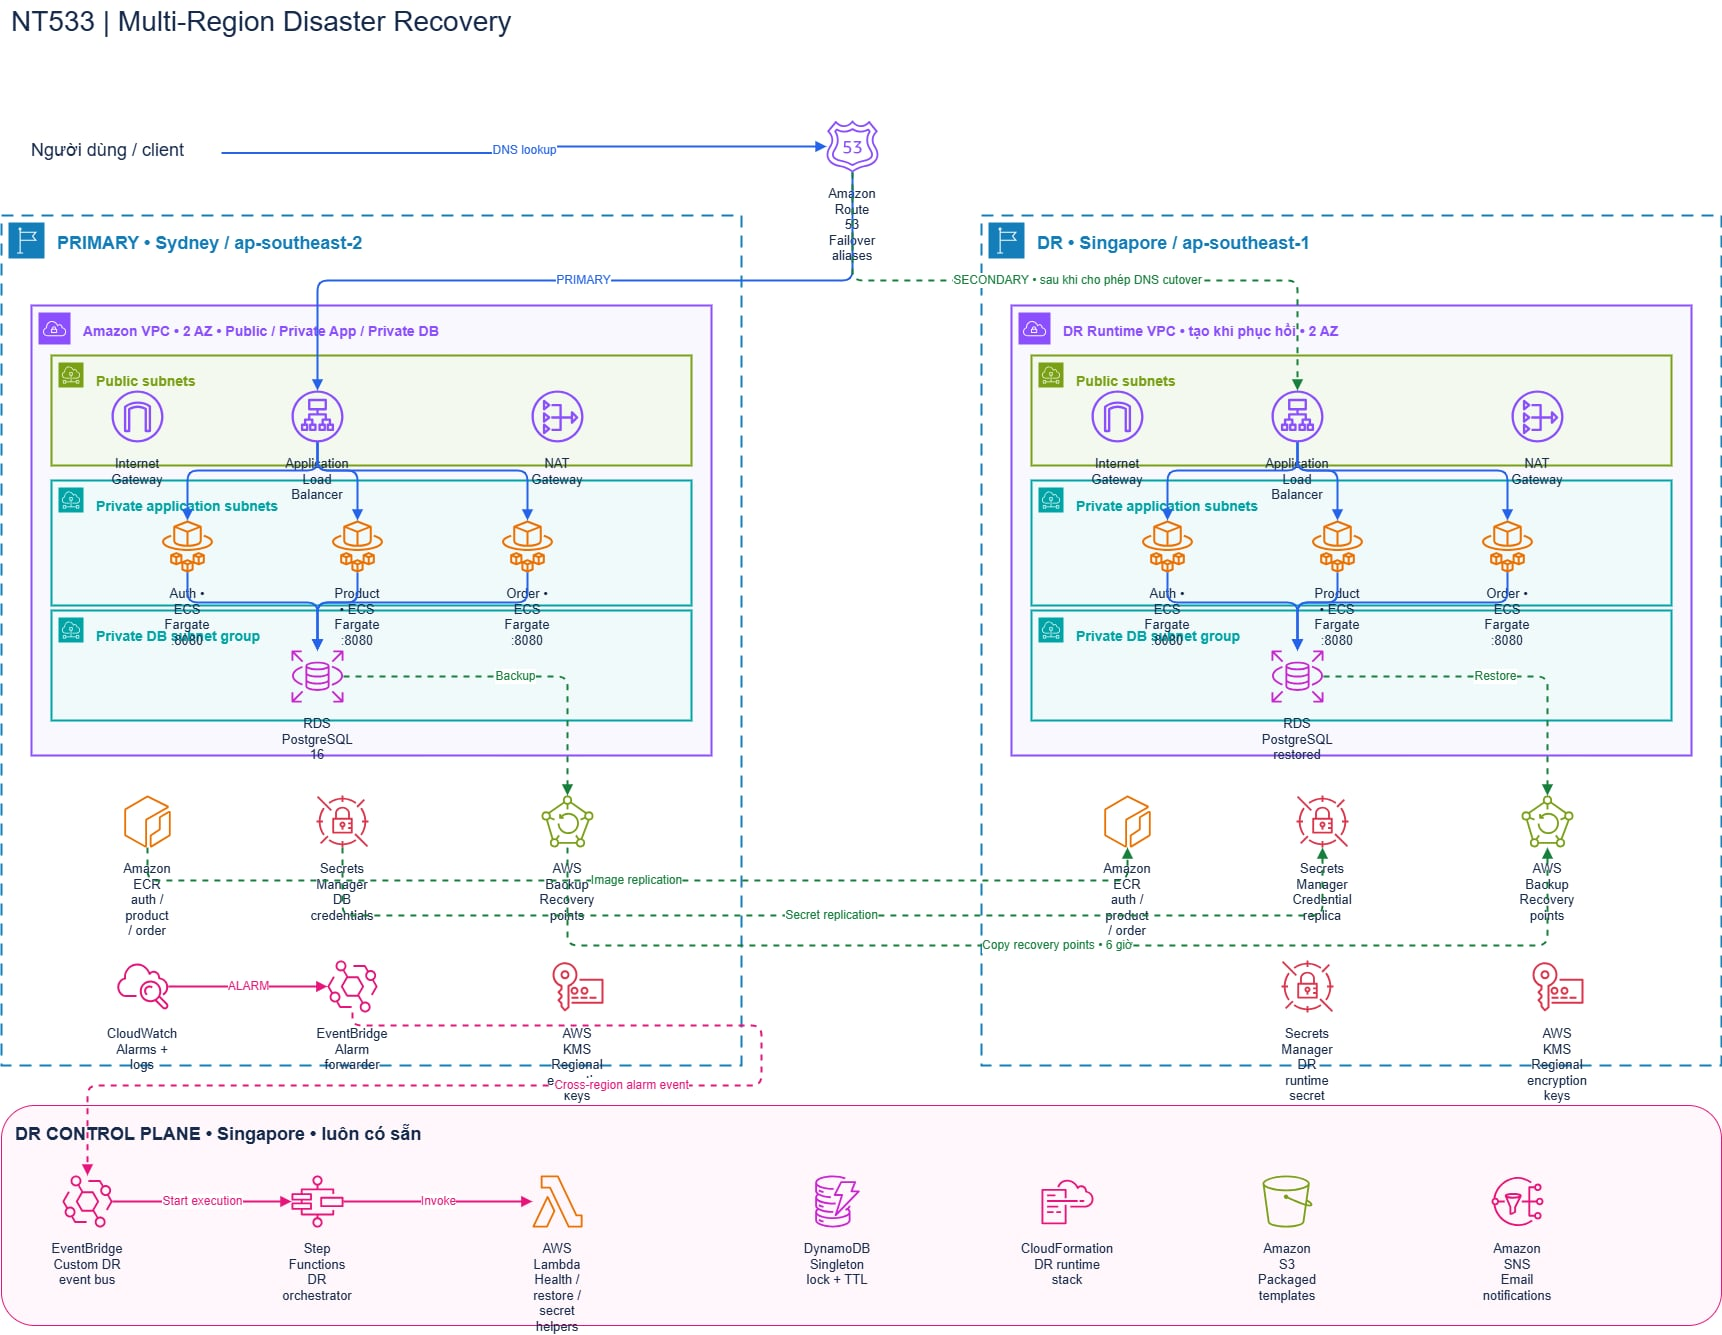
\includegraphics[width=\textwidth]{img/chapter3/nt533-architecture.jpg}
  \caption{Kiến trúc Multi-Region Disaster Recovery của NT533}
  \label{fig:architecture-overall}
\end{figure}

Luồng bình thường có thể tóm tắt như sau:

\begin{center}
\begin{tikzpicture}[node distance=9mm and 8mm, every node/.style={font=\small}, box/.style={draw, rounded corners, align=center, minimum height=9mm, fill=blue!5}, data/.style={draw, cylinder, shape border rotate=90, aspect=0.25, align=center, fill=green!8}, >=Latex]
\node[box] (client) {Client};
\node[box, right=of client] (dns) {Route 53\\PRIMARY};
\node[box, right=of dns] (alb) {ALB\\Sydney};
\node[box, right=of alb] (ecs) {ECS Fargate\\3 services};
\node[data, right=of ecs] (rds) {RDS\\PostgreSQL};
\draw[->] (client)--(dns);
\draw[->] (dns)--(alb);
\draw[->] (alb)--(ecs);
\draw[->] (ecs)--(rds);
\end{tikzpicture}
\end{center}

Song song với request path, AWS Backup tạo recovery point và copy sang Singapore; ECR replicate image theo prefix; Secrets Manager replicate credentials. Control plane DR tồn tại độc lập với runtime VPC, cho phép Region Singapore bắt đầu phục hồi ngay cả khi workload Sydney không truy cập được.

\section{Kiến trúc Primary Region}

\subsection{Mạng}

Template \path{cloudformation/primary/network.yaml} tạo VPC \texttt{10.10.0.0/16} trên hai AZ. Mỗi AZ có public, private application và private database subnet. Hai public subnet dùng chung route table có default route đến Internet Gateway. Hai application subnet dùng chung route table đi qua một NAT Gateway đặt tại public subnet thứ nhất. Hai database subnet dùng route table không có default route, tạo lớp mạng cô lập cho RDS.

Bảng~\ref{tab:primary-cidrs} tổng hợp giá trị từ \path{prod-primary.json}.

\begin{table}[H]
\centering
\caption{Phân hoạch CIDR tại Primary Region}
\label{tab:primary-cidrs}
\begin{tabularx}{\textwidth}{@{}l l X@{}}
\toprule
\textbf{Lớp mạng} & \textbf{CIDR} & \textbf{Vai trò} \\
\midrule
VPC & \texttt{10.10.0.0/16} & Không gian địa chỉ Primary \\
Public A/B & \texttt{10.10.0.0/24}, \texttt{10.10.1.0/24} & ALB, NAT Gateway \\
Application A/B & \texttt{10.10.10.0/24}, \texttt{10.10.11.0/24} & ECS task không có public IP \\
Database A/B & \texttt{10.10.20.0/24}, \texttt{10.10.21.0/24} & RDS subnet group, không có Internet route \\
\bottomrule
\end{tabularx}
\end{table}

Một NAT Gateway dùng chung giảm chi phí nhưng không đạt khả năng chịu lỗi AZ đầy đủ. Nếu AZ chứa NAT gặp sự cố, task ở cả hai application subnet có thể mất đường đến ECR, Secrets Manager hoặc AWS API qua Internet. VPC endpoint hoặc NAT theo AZ là phương án nâng cấp.

\subsection{Security Group}

ALB nhận HTTP/HTTPS từ Internet và chỉ egress đến ECS trên cổng 8080. ECS chỉ nhận cổng 8080 từ ALB; egress gồm HTTPS đến AWS API và PostgreSQL đến DB Security Group. RDS chỉ nhận 5432 từ ECS Security Group. Cấu hình thể hiện nguyên tắc least connectivity ở tầng mạng, dù egress HTTPS vẫn mở tới \texttt{0.0.0.0/0} vì hệ thống chưa dùng VPC endpoint.

\subsection{ALB và request routing}

ALB là internet-facing, trải trên hai public subnet. Nếu không có ACM certificate, listener HTTP trả fixed 404 mặc định và các path rule xử lý request. Nếu có certificate, HTTP redirect sang HTTPS và rule gắn vào HTTPS listener. Route \texttt{/auth} chuyển đến auth target group; \texttt{/product}, \texttt{/products} và \texttt{/health} đến product; \texttt{/order} đến order.

Health check của target group gọi \texttt{/health}. Vì cùng image được chạy với biến \texttt{SERVICE\_NAME} khác nhau và health endpoint luôn kiểm tra database, cả ba target group chỉ khỏe khi PostgreSQL có thể truy cập. Composite alarm dùng logic OR, do đó mất một service đã đủ kích hoạt quy trình xác nhận DR.

\subsection{ECS Fargate}

Ba task definition dùng CPU 256 và memory 512 theo parameter file, chạy Linux x86\_64, root filesystem chỉ đọc, ghi log vào CloudWatch Logs và lấy credentials từ Secrets Manager. Task execution role có managed policy chuẩn và quyền đọc đúng database secret. Task role không có application permission vì ứng dụng chỉ giao tiếp PostgreSQL qua mạng.

Parameter môi trường đặt \texttt{EcsDesiredCount=0}, do đó các service Primary được tạo trước và được scale lên sau khi image đã sẵn sàng. Cách tách hai bước giúp tránh ECS liên tục khởi động task khi image chưa được publish, nhưng yêu cầu quy trình triển khai phải có bước scale rõ ràng.

\subsection{RDS và secret}

RDS dùng PostgreSQL major version 16, lớp \texttt{db.t4g.micro}, 20 GiB gp3 mặc định, Single-AZ theo default, private subnet và storage encryption bằng KMS key riêng. Deletion policy và update-replace policy tạo snapshot; deletion protection lấy theo parameter và file production hiện đặt \texttt{false}. TLS được ép bằng parameter \texttt{rds.force\_ssl=1}. Secret tạo username \texttt{appadmin}, password ngẫu nhiên 32 ký tự và replica tại Singapore.

\subsection{Route 53 và monitoring}

Primary stack tạo failover alias PRIMARY cho \texttt{app.devopsss.site} và một Route~53 health check riêng gọi ALB DNS ở path \texttt{/health}. Alias đặt \texttt{EvaluateTargetHealth=true}; health check riêng chủ yếu phục vụ quan sát, không được gắn trực tiếp vào record. Monitoring stack tạo ba metric alarm, một composite alarm và dashboard theo dõi ALB, ECS, RDS, Route~53 và AWS Backup.

\section{Kiến trúc DR Region}

\subsection{Tài nguyên thường trực và tài nguyên theo nhu cầu}

Singapore không hoàn toàn ``chi phí bằng 0''. Các tài nguyên control plane và artifact vẫn tồn tại: S3 artifact bucket, backup vault và recovery point, KMS key, ECR repository, secret replica, Step Functions, Lambda, DynamoDB lock, EventBridge bus/rule, SQS DLQ, SNS và CloudWatch Logs. Phần có chi phí runtime đáng kể hơn gồm NAT Gateway, ALB, ECS task và RDS chỉ được tạo hoặc khởi chạy khi DR.

\begin{table}[H]
\centering
\caption{Trạng thái tài nguyên DR trước và sau kích hoạt}
\label{tab:dr-resource-state}
\begin{tabularx}{\textwidth}{@{}p{2.8cm}p{3.4cm}p{4cm}X@{}}
\toprule
\textbf{Tài nguyên} & \textbf{Bình thường} & \textbf{Khi kích hoạt DR} & \textbf{Tác động chi phí} \\
\midrule
Backup vault/KMS & Tồn tại, lưu recovery point & Dùng làm nguồn restore & Chi phí lưu trữ và request thường trực \\
ECR & Ba repository tồn tại & ECS pull image replicated & Chi phí lưu image; không có compute \\
Control plane & Step Functions, Lambda, DynamoDB, EventBridge, SNS tồn tại & Phát sinh execution/request & Chi phí chờ thấp, chủ yếu theo sử dụng \\
VPC/NAT & Không có runtime VPC & CloudFormation tạo VPC, subnets, một NAT & NAT có phí theo giờ và dữ liệu trong thời gian DR \\
ALB & Không tồn tại & Tạo internet-facing ALB và 3 target group & Phí ALB bắt đầu khi stack được tạo \\
ECS & Không có cluster runtime & Tạo service desired count 0, sau đó scale lên 1 mỗi service & Chỉ trả Fargate khi task chạy \\
RDS & Không có instance DR & AWS Backup restore \texttt{db.t4g.micro} & Chi phí DB bắt đầu sau restore \\
Route 53 SECONDARY & Không tồn tại & Chỉ UPSERT nếu không skip DNS & Thay đổi traffic là rủi ro vận hành \\
\bottomrule
\end{tabularx}
\end{table}

\subsection{DR runtime stack}

VPC DR dùng CIDR \texttt{10.20.0.0/16} với cấu trúc subnet tương tự Primary. Root stack tạo network, security, ALB, IAM, ECS và dashboard. RDS không nằm trong CloudFormation stack vì được AWS Backup restore riêng. ECS service được tạo với desired count 0; runtime secret ban đầu chứa trạng thái \texttt{pending-restore}. Chỉ sau khi database available và secret được cập nhật, Step Functions mới scale dịch vụ.

Thiết kế này tránh task khởi động liên tục với endpoint chưa tồn tại. Nó cũng tạo ranh giới cleanup: phải xóa RDS restore riêng trước hoặc sau khi xóa runtime stack. Script cleanup xử lý đúng thứ tự, đồng thời yêu cầu record SECONDARY không còn tồn tại.

\section{Cơ chế sao lưu và phục hồi dữ liệu}

Backup plan chạy \texttt{cron(0 0/6 ? * * *)}, có start window 60 phút, completion window 360 phút và retention bảy ngày ở cả nguồn lẫn bản copy. Backup selection tham chiếu chính xác ARN RDS Primary. Backup service role dùng managed policy và quyền KMS cần thiết cho hai key.

Khi chạy DR, Lambda \texttt{find-recovery-point} phân trang toàn bộ recovery point kiểu RDS tại DR vault, chỉ giữ trạng thái \texttt{COMPLETED}, khớp ARN hoặc database identifier và chọn \texttt{CreationDate} mới nhất. Lambda \texttt{start-restore} đọc restore metadata, loại bỏ các field không phù hợp, ghi đè DB identifier, class, subnet group, Security Group, Multi-AZ và deletion protection rồi gọi \texttt{StartRestoreJob}.

Chu kỳ backup sáu giờ ảnh hưởng trực tiếp đến lượng dữ liệu có khả năng mất khi xảy ra sự cố. Ngoài chu kỳ này, thời gian tạo backup và copy liên vùng cũng quyết định recovery point mới nhất có sẵn tại Singapore. Script kiểm thử dữ liệu được thiết kế để chỉ chọn recovery point tạo sau bản ghi kiểm thử; tuy nhiên lần chạy được truy vết không còn output đối chiếu record, nên báo cáo không kết luận kết quả kiểm tra dữ liệu đầu cuối.

\section{Quy trình tự động DR}

State machine có 57 trạng thái. Có thể nhóm thành chín giai đoạn như Hình~\ref{fig:dr-sequence}.

\begin{figure}[H]
\centering
\begin{tikzpicture}[node distance=6mm, every node/.style={font=\scriptsize}, drstep/.style={draw, rounded corners, align=center, text width=4.2cm, minimum height=8mm, fill=blue!5}, >=Latex]
\node[drstep] (trigger) {1. Validate trigger và acquire DynamoDB lock};
\node[drstep, below=of trigger] (confirm) {2. SNS, chờ 90 giây, kiểm tra lại Primary};
\node[drstep, below=of confirm] (stack) {3. Create DR CloudFormation stack và parse outputs};
\node[drstep, below=of stack] (backup) {4. Chọn recovery point và start RDS restore};
\node[drstep, below=of backup] (db) {5. Poll restore/RDS đến trạng thái available};
\node[drstep, below=of db] (secret) {6. Ghép endpoint mới với credentials replica};
\node[drstep, below=of secret] (ecs) {7. Scale ba ECS service song song};
\node[drstep, below=of ecs] (health) {8. Poll target groups, tối đa khoảng 15 phút};
\node[drstep, below=of health] (cutover) {9. Kiểm tra lại Primary, tùy chọn DNS, SNS, release lock};
\draw[->] (trigger)--(confirm);
\draw[->] (confirm)--(stack);
\draw[->] (stack)--(backup);
\draw[->] (backup)--(db);
\draw[->] (db)--(secret);
\draw[->] (secret)--(ecs);
\draw[->] (ecs)--(health);
\draw[->] (health)--(cutover);
\end{tikzpicture}
\caption{Các giai đoạn logic của quy trình DR}
\label{fig:dr-sequence}
\end{figure}

\subsection{Đường thành công}

Workflow chấp nhận trigger \texttt{alarm} hoặc \texttt{manual-test}. Sau khi chiếm lock, hệ thống gửi thông báo, chờ 90 giây và kiểm tra Primary. Với test mode, Lambda trả trạng thái simulated failure; với alarm thật, Lambda đọc cả metric và composite alarm ở Sydney. Nếu Primary phục hồi, workflow thông báo hủy và giải phóng lock.

Nếu sự cố còn tồn tại, workflow tạo stack \texttt{prod-dr-runtime-production} với \texttt{OnFailure=ROLLBACK}. Sau \texttt{CREATE\_COMPLETE}, outputs bắt buộc được parse. Recovery point mới nhất được restore; job và RDS được poll riêng đến khi hoàn tất. Runtime secret được cập nhật, ba service scale song song, rồi target groups được kiểm tra mỗi 30 giây. Khi khỏe, Primary được kiểm tra lần cuối. DNS chỉ thay đổi nếu Primary vẫn lỗi và cả hai trường input skip DNS đều không true.

\subsection{Đường thất bại và rollback}

Các Task quan trọng có Catch chuyển đến \texttt{NotifyFailure}; workflow gửi SNS, giải phóng lock và kết thúc \texttt{Fail}. Stack creation dùng rollback của CloudFormation. ECS service dùng deployment circuit breaker. Nếu restore recovery point mới nhất trả về \texttt{FAILED} hoặc \texttt{ABORTED}, workflow chọn recovery point kế tiếp chưa thử. Khi hết recovery point, workflow ghi stage \texttt{data-restore}, gửi SNS và chuyển manual recovery. Lỗi CloudFormation được giữ lại cùng stack events để điều tra; cleanup là quy trình riêng có xác nhận, tránh xóa bằng chứng hoặc dữ liệu cần phục hồi.

\subsection{Retry và timeout}

Retry tập trung vào throttling và lỗi dịch vụ tạm thời, với exponential backoff. Workflow timeout mặc định 43.200 giây. ALB health loop khởi tạo counter 0, kiểm tra sau mỗi 30 giây và timeout khi counter đạt 30; thời gian thực tế xấp xỉ 15--15,5 phút tùy cách tính lần đầu. CloudFormation và RDS loops không có counter riêng, nhưng bị giới hạn bởi timeout toàn workflow.

\section{Bảo mật và IAM}

Mỗi Lambda có role riêng. Manage-lock chỉ có Get/Put/Delete trên đúng table; find-recovery-point chỉ list trong đúng vault; update-secret chỉ đọc secret nguồn theo tên và ghi runtime secret theo prefix. Một số API không hỗ trợ resource-level permission hoặc code dùng wildcard, như \texttt{DescribeAlarms}, \texttt{DescribeDBInstances} và \texttt{DescribeTargetHealth}.

CloudFormation execution role có quyền dựng runtime hạ tầng; Step Functions chỉ được pass đúng execution role và restore role với điều kiện service. Backup restore role dùng managed policy cho restore và KMS decrypt/create grant. S3 bucket chặn public access, bật versioning và từ chối HTTP. ECR immutable, scan on push. SNS dùng customer-managed KMS key. DynamoDB và SQS bật mã hóa server-side.

Hai giới hạn bảo mật đáng chú ý. Thứ nhất, parameter JSON chứa AWS account ID, ARN, hosted zone và email; đây không phải password nhưng là metadata môi trường, nên được chuyển sang cấu hình riêng khi công khai dự án. Thứ hai, endpoint ứng dụng trả trường \texttt{detail} chứa exception database cho client khi lỗi, có thể tiết lộ hostname hoặc thông tin nội bộ; production API nên trả lỗi chung và giữ chi tiết trong log.

\section{Phân tích tối ưu chi phí}

Thiết kế giảm chi phí bằng ba quyết định: không duy trì RDS tại DR; không chạy ECS task tại DR; chỉ tạo NAT Gateway và ALB khi cần. Các artifact có chi phí thấp hơn compute liên tục được giữ sẵn để rút ngắn thời gian chuẩn bị. DynamoDB dùng on-demand; Lambda, Step Functions và EventBridge tính theo sử dụng; ECR và backup tính theo dung lượng.

Đánh đổi là RTO phụ thuộc thời gian CloudFormation và RDS restore. Single NAT và Single-AZ RDS giảm chi phí nhưng hạ khả năng chịu lỗi trong từng Region. Ba service dùng cùng image và cùng database giúp demo đơn giản, nhưng không đại diện đầy đủ cho microservices độc lập. Vì vậy, kiến trúc phù hợp đồ án và workload chấp nhận downtime hàng chục phút; không nên áp dụng nguyên trạng cho hệ thống có RTO vài phút hoặc yêu cầu HA nghiêm ngặt.


\chapter{TRIỂN KHAI VÀ THỰC NGHIỆM}
\label{c:lienquan}
\section{Môi trường triển khai}

Primary Region của hệ thống đặt tại Sydney (\texttt{ap-southeast-2}); DR và automation đặt tại Singapore (\texttt{ap-southeast-1}). Hạ tầng được triển khai bằng AWS CloudFormation nested stack, AWS CLI và PowerShell. Ứng dụng chạy trên Python 3.12, được đóng gói thành container và lắng nghe tại cổng 8080.

\begin{table}[H]
\centering
\caption{Cấu hình môi trường chính}
\label{tab:environment}
\begin{tabularx}{\textwidth}{@{}l l X@{}}
\toprule
\textbf{Hạng mục} & \textbf{Giá trị} & \textbf{Mô tả} \\
\midrule
Primary Region & \texttt{ap-southeast-2} & Sydney, chạy workload chính \\
DR Region & \texttt{ap-southeast-1} & Singapore, lưu artifact và phục hồi theo nhu cầu \\
Database & PostgreSQL 16, \texttt{db.t4g.micro} & RDS mã hóa, private subnet \\
Container & Python 3.12, cổng 8080 & Ba ECS Fargate service \\
ECS task size & 256 CPU, 512 MiB & Cấu hình cho ứng dụng demo \\
Backup & Mỗi 6 giờ, giữ 7 ngày & Copy recovery point sang Singapore \\
DR desired count & 1 mỗi service sau restore & Scale sau khi database sẵn sàng \\
Workflow timeout & 43.200 giây & Giới hạn tối đa 12 giờ \\
DNS test mode & Bỏ qua cutover & Không tác động traffic production \\
\bottomrule
\end{tabularx}
\end{table}

Thông tin kết nối database được quản lý bằng AWS Secrets Manager. Các giá trị môi trường như ARN, hosted zone và email được truyền qua parameter; báo cáo không trình bày credential hoặc nội dung secret.

\section{Quy trình triển khai}

\subsection{Kiểm tra cú pháp}

Trước khi deploy, nhóm chạy \texttt{validate.ps1} để kiểm tra toàn bộ template bằng \texttt{cfn-lint} tại cả hai Region, đồng thời compile bytecode cho Lambda và ứng dụng Python.

\begin{lstlisting}[language=PowerShell,caption={Kiểm tra template và mã nguồn},label={lst:validate}]
.\cloudformation\scripts\validate.ps1
\end{lstlisting}

\subsection{Bootstrap và đóng gói artifact}

Regional baseline được triển khai tại Sydney và Singapore để tạo S3 artifact bucket, KMS key và AWS Backup vault. Ba ECR repository đích được chuẩn bị tại Singapore. Script \texttt{package.ps1} đóng gói các nested template; DR runtime template được lưu theo release version để workflow luôn tham chiếu một artifact hạ tầng xác định.

\begin{lstlisting}[language=PowerShell,caption={Đóng gói nested template},label={lst:package}]
.\cloudformation\scripts\package.ps1 `
  -PrimaryArtifactBucket <PRIMARY_BUCKET> `
  -DrArtifactBucket <DR_BUCKET> `
  -ReleaseVersion v1.0.X
\end{lstlisting}

\subsection{Triển khai Primary và publish image}

Primary stack tạo VPC, ALB, ECS, RDS, ECR, AWS Backup và monitoring tại Sydney. Các ECS service ban đầu có desired count bằng 0; sau khi image được build và push lên ECR, service được scale theo quy trình triển khai. Cross-Region replication chuyển image sang Singapore để DR runtime có thể pull image mà không phụ thuộc Primary Region.

\begin{lstlisting}[language=PowerShell,caption={Publish image ứng dụng},label={lst:images}]
.\cloudformation\scripts\publish-images.ps1 `
  -AccountId <AWS_ACCOUNT_ID> `
  -ImageTag v1 `
  -RepositoryPrefix prod
\end{lstlisting}

ECR bật immutable tag, vì vậy mỗi bản phát hành cần sử dụng tag mới. Trước khi kiểm thử DR, nhóm cần xác nhận image đã xuất hiện tại Singapore.

\subsection{Triển khai automation}

Automation stack được triển khai tại Singapore sau khi các ARN của Primary alarm, source database, DR backup vault và runtime template đã sẵn sàng. EventBridge tại Sydney chuyển sự kiện alarm sang custom event bus tại Singapore; Step Functions tiếp nhận sự kiện và điều phối toàn bộ quá trình phục hồi.

\section{Kịch bản kiểm thử DR}

Nhóm sử dụng execution \path{real-data-dr-20260930-214735}, bắt đầu lúc 14:49:42 UTC ngày 30/09/2026. Kịch bản chạy theo chế độ an toàn với các giá trị sau:

\begin{itemize}
  \item trigger: \texttt{manual-test};
  \item mô phỏng sự cố và test mode: bật;
  \item chuyển Route~53: bỏ qua.
\end{itemize}

Nhờ đó workflow đi qua toàn bộ quá trình tạo runtime, restore database, scale ECS và kiểm tra ALB nhưng không thay đổi DNS production.

Quá trình thực nghiệm diễn ra theo thứ tự:

\begin{enumerate}
  \item khởi tạo execution và chiếm DynamoDB lock;
  \item xác nhận điều kiện DR, sau đó tạo stack \texttt{prod-dr-runtime-production};
  \item chọn recovery point trong vault Singapore và khởi tạo AWS Backup restore job;
  \item chờ RDS ở trạng thái \texttt{available}, cập nhật runtime secret;
  \item scale ba service \texttt{auth}, \texttt{product} và \texttt{order} lên desired count 1;
  \item kiểm tra ba target group đến khi tất cả healthy;
  \item bỏ qua Route~53 cutover, gửi thông báo hoàn tất và giải phóng lock.
\end{enumerate}

\begin{table}[H]
\centering
\caption{Kết quả các hạng mục kiểm thử}
\label{tab:test-status}
\begin{tabularx}{\textwidth}{@{}p{4cm}p{5cm}X@{}}
\toprule
\textbf{Hạng mục} & \textbf{Cách thực hiện} & \textbf{Kết quả} \\
\midrule
Khởi tạo DR workflow & Manual safe test & Thành công \\
Tạo DR runtime & CloudFormation nested stack & Thành công \\
Restore RDS & AWS Backup recovery point tại Singapore & Thành công \\
Khởi chạy ECS & Scale ba service sau khi RDS available & Thành công \\
ALB health gate & Hai lần gọi Lambda \texttt{check-alb} & Thành công \\
\bottomrule
\end{tabularx}
\end{table}

Quá trình triển khai và thực hiện kịch bản DR được nhóm ghi lại dưới dạng video demo. Timeline định lượng trong báo cáo được đối chiếu độc lập từ lịch sử dịch vụ AWS.

\section{Kết quả thực nghiệm}

CloudTrail ghi nhận execution bắt đầu lúc \texttt{14:49:42 UTC}. CloudFormation runtime hoàn tất lúc \texttt{14:58:46.717 UTC}. AWS Backup restore job \texttt{1816ab82-...-013f29ece4bf} chạy từ \texttt{14:58:51.187 UTC} đến \texttt{15:07:18.723 UTC} với trạng thái \texttt{COMPLETED}. Ba ECS service được scale lúc \texttt{15:07:55 UTC}. Lần kiểm tra ALB thứ hai hoàn tất lúc \texttt{15:08:56.762 UTC}; ngay sau đó workflow kiểm tra Primary lần cuối và giải phóng lock. Bảng~\ref{tab:experiment-milestones} trích trực tiếp các trường có giá trị minh chứng từ dữ liệu AWS; Account ID và ARN đầy đủ không được đưa vào báo cáo.

\begin{table}[H]
\centering
\caption{Các mốc chính của lần thực nghiệm DR ngày 30/09/2026}
\label{tab:experiment-milestones}
\small
\begin{tabularx}{\textwidth}{@{}p{4.2cm}p{3.4cm}X@{}}
\toprule
\textbf{Mốc quan sát} & \textbf{Thời điểm UTC} & \textbf{Nguồn và giá trị minh chứng} \\
\midrule
\texttt{StartExecution} & 14:49:42.000 & CloudTrail; execution \texttt{real-data-dr-20260930-214735} \\
CloudFormation \texttt{CREATE\_COMPLETE} & 14:58:46.717 & Stack \texttt{prod-dr-runtime-production} \\
AWS Backup restore bắt đầu & 14:58:51.187 & Restore job \texttt{1816ab82-...-013f29ece4bf} \\
AWS Backup restore hoàn tất & 15:07:18.723 & Trạng thái \texttt{COMPLETED}, tiến độ \texttt{100.00\%} \\
RDS \texttt{available} được quan sát & 15:07:53.939 & Lambda \texttt{update-secret}; DB \texttt{prod-dr-restored-db} \\
ECS bắt đầu scale & 15:07:55.000 & Cluster \texttt{prod-dr-dr-ecs}; ba service lên desired count 1 \\
Các ALB target group healthy & 15:08:56.762 & Lần gọi \texttt{check-alb} thứ hai; ba target group qua health gate \\
Release lock hoàn tất & 15:08:59.230 & Lambda \texttt{manage-lock}; bước cuối quan sát được của workflow \\
\bottomrule
\end{tabularx}
\end{table}

\begin{table}[H]
\centering
\caption{Thời lượng các giai đoạn của lần thực nghiệm DR}
\label{tab:experiment-timeline}
\begin{tabularx}{\textwidth}{@{}p{4.2cm}p{3.2cm}p{3.2cm}r@{}}
\toprule
\textbf{Giai đoạn} & \textbf{Bắt đầu UTC} & \textbf{Kết thúc UTC} & \textbf{Thời lượng} \\
\midrule
Chuẩn bị trước khi tạo runtime & 14:49:42.000 & 14:51:15.738 & 1 phút 33,738 giây \\
Tạo DR runtime stack & 14:51:15.738 & 14:58:46.717 & 7 phút 30,979 giây \\
Chuyển tiếp sang restore job & 14:58:46.717 & 14:58:51.187 & 4,470 giây \\
Restore RDS bằng AWS Backup & 14:58:51.187 & 15:07:18.723 & 8 phút 27,536 giây \\
Chờ workflow quan sát RDS available & 15:07:18.723 & 15:07:53.939 & 35,216 giây \\
Cập nhật secret và bắt đầu scale ECS & 15:07:53.939 & 15:07:55.000 & 1,061 giây \\
Scale ECS đến ALB healthy & 15:07:55.000 & 15:08:56.762 & 1 phút 1,762 giây \\
ALB healthy đến release lock & 15:08:56.762 & 15:08:59.230 & 2,468 giây \\
\midrule
\textbf{Tổng: workflow start đến ALB healthy} & \textbf{14:49:42.000} & \textbf{15:08:56.762} & \textbf{19 phút 14,762 giây} \\
Tổng: workflow start đến release lock & 14:49:42.000 & 15:08:59.230 & 19 phút 17,230 giây \\
\bottomrule
\end{tabularx}
\end{table}

\begin{figure}[H]
\centering
\begin{tikzpicture}
\begin{axis}[
  xbar,
  width=0.86\textwidth,
  height=7.2cm,
  xlabel={Thời lượng (giây)},
  xmin=0,
  xmax=620,
  bar width=10pt,
  symbolic y coords={Kích hoạt ứng dụng,Restore RDS,Chuyển tiếp restore,Tạo DR runtime,Chuẩn bị workflow},
  ytick=data,
  y dir=reverse,
  nodes near coords,
  nodes near coords align={horizontal},
  every node near coord/.append style={font=\scriptsize},
  tick label style={font=\small},
  label style={font=\small},
  grid=major,
  grid style={draw=gray!20},
  axis line style={draw=gray!60},
  enlarge y limits=0.12
]
\addplot[fill=blue!55,draw=blue!70!black] coordinates {
  (98.039,Kích hoạt ứng dụng)
  (507.536,Restore RDS)
  (4.470,Chuyển tiếp restore)
  (450.979,Tạo DR runtime)
  (93.738,Chuẩn bị workflow)
};
\end{axis}
\end{tikzpicture}
\caption{Thời lượng các giai đoạn từ workflow start đến ALB healthy}
\label{fig:recovery-stage-duration}
\end{figure}

Kết quả trong Hình~\ref{fig:recovery-stage-duration} cho thấy phần lớn thời gian tập trung ở hai giai đoạn: tạo runtime CloudFormation và restore RDS. Sau khi restore job hoàn tất, hệ thống cần thêm khoảng 1 phút 38 giây để quan sát RDS available, cập nhật secret, scale ECS và đưa toàn bộ target group về trạng thái healthy.

Thời gian 19 phút 17 giây phù hợp với ghi nhận ban đầu ``khoảng 21 phút'', nhưng có ranh giới đo rõ hơn: từ API \texttt{StartExecution} đến khi bước release lock ngay trước trạng thái thành công hoàn tất. Giá trị này phản ánh thời gian workflow trong điều kiện safe test của đồ án, không phải cam kết SLA của hệ thống production.

\section{Phân tích thời gian phục hồi}

CloudFormation bắt đầu tạo runtime sau khoảng 1 phút 34 giây, tương ứng với bước lock và confirmation window đầu workflow. Runtime stack cần khoảng 7 phút 31 giây để tạo VPC, NAT Gateway, security group, ALB, ECS service zero-count và monitoring. Đây là phần có thể rút ngắn nếu chuyển một số tài nguyên sang mô hình Pilot Light, nhưng đổi lại Singapore sẽ phát sinh chi phí thường trực cao hơn.

RDS restore mất khoảng 8 phút 28 giây và là giai đoạn dài nhất. Thời gian này phụ thuộc kích thước recovery point, DB class và tải của dịch vụ AWS Backup/RDS. Sau restore, việc scale ba ECS service diễn ra song song. Health gate chỉ thành công ở lần kiểm tra thứ hai, khoảng một phút sau khi scale service.

Kịch bản không thực hiện Route~53 cutover, vì vậy timeline không bao gồm thời gian thay đổi record, trạng thái \texttt{INSYNC} hoặc cache DNS phía client. Chu kỳ backup sáu giờ vẫn là yếu tố chính ảnh hưởng đến độ mới của dữ liệu phục hồi. Output đối chiếu record của script cũ không còn, nên lần thực nghiệm này chỉ kết luận thành công ở mức hạ tầng, database restore và application health.

\section{Giới hạn thực nghiệm}

Thực nghiệm được phân tích từ một execution nên chưa thể đánh giá độ biến thiên giữa nhiều lần chạy. State machine đã được xóa sau khi demo, làm execution history gốc không còn truy xuất được; timestamp cuối được xác định từ Lambda release lock ngay trước trạng thái \texttt{DrSucceeded}. Kịch bản cũng không đo downtime bằng probe bên ngoài và không cutover DNS.

Các lần kiểm thử sau nên tự động lưu execution history, CloudFormation events, restore job, target health và probe log vào S3 theo execution ID. Khi có nhiều mẫu trong cùng điều kiện, nhóm mới có thể so sánh độ ổn định của thời gian phục hồi và đánh giá ảnh hưởng của kích thước database.


\chapter{ĐÁNH GIÁ VÀ HƯỚNG PHÁT TRIỂN}
\label{c:danhgia}
\section{Kết quả đạt được}

Đồ án đã xây dựng được chuỗi kỹ thuật cốt lõi của chiến lược Backup and Restore: hạ tầng Primary tại Sydney, sao chép artifact sang Singapore, control plane DR, runtime stack theo nhu cầu, RDS restore, cập nhật secret, scale ECS và health gate trước khi cho phép cutover.

Lần thực nghiệm ngày 30/09/2026 cho thấy workflow có thể tạo hoàn chỉnh runtime tại Singapore, khôi phục RDS và đưa ba target group về trạng thái healthy. Application health đạt sau khoảng 19 phút 15 giây; bước cuối ngay trước trạng thái thành công hoàn tất sau khoảng 19 phút 17 giây. Kịch bản được thực hiện ở chế độ an toàn nên Route~53 không bị thay đổi.

\begin{table}[H]
\centering
\caption{Đối chiếu mục tiêu và kết quả đạt được}
\label{tab:objectives}
\begin{tabularx}{\textwidth}{@{}p{4.2cm}p{3cm}X@{}}
\toprule
\textbf{Mục tiêu} & \textbf{Kết quả} & \textbf{Nhận xét} \\
\midrule
IaC đa vùng & Hoàn thành & Nested CloudFormation cho Primary, DR và automation \\
Backup/copy RDS & Hoàn thành & Recovery point Singapore được restore thành công \\
Replicate image/secret & Hoàn thành & Artifact cần thiết có mặt tại DR Region \\
Tự động dựng DR runtime & Hoàn thành & Runtime stack đạt \texttt{CREATE\_COMPLETE} \\
Khởi chạy ứng dụng DR & Hoàn thành & Ba ECS service được scale và ALB health gate thành công \\
Kiểm tra dữ liệu record & Chưa kết luận & Không còn output đối chiếu record của lần chạy \\
DNS cutover & Không thuộc safe test & Workflow chủ động bỏ qua Route~53 \\
Cleanup & Hoàn thành & RDS restore và runtime stack đã được xóa sau test \\
\bottomrule
\end{tabularx}
\end{table}

\section{Đánh giá kiến trúc}

Ưu điểm chính của hệ thống là mức độ tự động hóa cao trong khi chi phí standby được giữ thấp. Singapore lưu trữ backup, image, secret và control plane nhưng không duy trì RDS, ALB, NAT Gateway hoặc ECS task của workload DR trong trạng thái bình thường. Khi được kích hoạt, workflow tạo đúng các tài nguyên cần thiết theo thứ tự phụ thuộc.

Việc sử dụng CloudFormation giúp hạ tầng có thể tái tạo và review. DynamoDB lock ngăn nhiều execution cùng sửa một tập tài nguyên. Workflow kiểm tra Primary trước và sau khi dựng DR, chỉ scale ECS sau khi RDS available, đồng thời yêu cầu cả ba target group healthy trước nhánh DNS. Chế độ safe test cho phép diễn tập phần lớn quy trình mà không tác động traffic production.

Về bảo mật, ECS task nằm trong private subnet và không được cấp public IP; RDS không public; kết nối database được quản lý bằng Secrets Manager; dữ liệu, backup và artifact được mã hóa bằng KMS. IAM role được tách theo chức năng của Step Functions, Lambda, CloudFormation và AWS Backup.

\section{Hạn chế}

\subsection{Khả năng sẵn sàng trong từng Region}

Primary và DR runtime sử dụng một NAT Gateway; RDS mặc định Single-AZ. Thiết kế này phù hợp mục tiêu tối ưu chi phí của đồ án nhưng chưa cung cấp HA đầy đủ trước sự cố ở phạm vi Availability Zone. Môi trường production quan trọng nên cân nhắc NAT Gateway theo AZ và RDS Multi-AZ.

\subsection{DNS cutover}

Workflow có khả năng tạo record Route~53 SECONDARY, nhưng input EventBridge và kịch bản test đều mặc định bỏ qua thao tác này. Hiện tại hệ thống phù hợp với mô hình tự động phục hồi hạ tầng, sau đó người vận hành quyết định cutover. Nếu bật chuyển DNS tự động, cần bổ sung bước phê duyệt hoặc policy rõ ràng, theo dõi \texttt{INSYNC} và probe bên ngoài AWS.

\subsection{Failback và dữ liệu}

Đồ án chưa có workflow failback từ Singapore về Sydney. Nếu ứng dụng nhận dữ liệu mới sau cutover, việc quay lại Primary cần quy trình backup hoặc replication ngược, kiểm tra consistency và kiểm soát thời điểm dừng ghi. Cleanup đơn thuần không thể thay thế failback.

Output của bước đối chiếu record trong kịch bản cũ không còn được lưu, nên kết quả hiện tại không dùng để khẳng định dữ liệu ứng dụng đầu cuối đã được xác minh. Lần thử tiếp theo cần lưu ID record trước backup và kết quả truy vấn sau restore.

\subsection{Idempotency và vận hành}

DynamoDB lock giảm nguy cơ chạy đồng thời, nhưng restore token được sinh ngẫu nhiên cho mỗi lần gọi Lambda. Một retry xảy ra sau khi AWS Backup đã nhận request nhưng trước khi Lambda nhận response có thể tạo cửa sổ không nhất quán. Token nên được tạo xác định từ execution ID và recovery point.

Workflow giữ lại tài nguyên khi thất bại để phục vụ điều tra. Cách làm này an toàn cho dữ liệu nhưng có thể phát sinh chi phí nếu không có cảnh báo và cleanup kịp thời. Cần alarm cho execution thất bại, lock tồn tại quá lâu và runtime hoạt động vượt thời gian cho phép.

\subsection{Ứng dụng demo}

Ba service dùng chung code, image và PostgreSQL; auth và order chưa có nghiệp vụ độc lập. Ứng dụng chưa có authentication, WAF, rate limiting hoặc distributed tracing. Response HTTP 500 còn trả chi tiết exception database. Các điểm này không cản trở mục tiêu kiểm thử DR nhưng cần được hardening trước khi áp dụng cho production.

\section{Hướng phát triển}

\begin{enumerate}
  \item Tự động lưu execution history, stack events, restore job và probe log vào S3 theo execution ID.
  \item Thực hiện nhiều DR run trong cùng điều kiện để đánh giá độ ổn định của timeline.
  \item Xây dựng quy trình failback và kiểm tra dữ liệu hai chiều.
  \item Bổ sung manual approval hoặc policy tự động trước Route~53 cutover.
  \item Tăng HA trong Region bằng RDS Multi-AZ và kiến trúc NAT theo AZ khi yêu cầu độ tin cậy cao hơn.
  \item Hardening ứng dụng: lỗi trả về an toàn, authentication, WAF, TLS và tracing.
  \item Đánh giá Pilot Light hoặc Warm Standby nếu yêu cầu thời gian phục hồi thấp hơn mức Backup and Restore hiện tại.
\end{enumerate}

Mỗi hướng tối ưu đều làm thay đổi chi phí và độ phức tạp vận hành. Vì vậy, kiến trúc tương lai cần được lựa chọn dựa trên mức độ quan trọng của workload thay vì chỉ tối thiểu hóa một chỉ số kỹ thuật.

\section{Kết luận}

Đồ án đã xây dựng và kiểm thử được hệ thống Disaster Recovery đa vùng trên AWS theo chiến lược Backup and Restore. Workload chính chạy tại Sydney; Singapore lưu các artifact phục hồi và chỉ tạo runtime khi workflow được kích hoạt. Step Functions tự động phối hợp CloudFormation, AWS Backup, RDS, Secrets Manager, ECS và ALB để đưa ứng dụng dự phòng về trạng thái healthy.

Kết quả thực nghiệm ghi nhận application health sau khoảng 19 phút 15 giây và đường workflow hoàn tất sau khoảng 19 phút 17 giây trong chế độ safe test. Mô hình cho thấy khả năng giảm đáng kể chi phí standby so với việc chạy hai Region đầy đủ, với đánh đổi là thời gian tạo hạ tầng và restore database. Đây là nền tảng phù hợp để tiếp tục phát triển failback, HA trong Region và hệ thống đo lường tự động cho các lần diễn tập tiếp theo.

\clearpage

\phantomsection
\addcontentsline{toc}{chapter}{DANH MỤC TÀI LIỆU THAM KHẢO}
\begin{thebibliography}{99}
\bibitem{aws-dr-objectives} Amazon Web Services. \textit{Disaster Recovery (DR) Objectives}. 2026. \url{https://docs.aws.amazon.com/wellarchitected/latest/reliability-pillar/disaster-recovery-dr-objectives.html}
\bibitem{aws-dr-options} Amazon Web Services. \textit{Disaster Recovery Options in the Cloud}. 2026. \url{https://docs.aws.amazon.com/whitepapers/latest/disaster-recovery-workloads-on-aws/disaster-recovery-options-in-the-cloud.html}
\bibitem{aws-well-architected-reliability} Amazon Web Services. \textit{AWS Well-Architected Framework: Reliability Pillar}. 2026. \url{https://docs.aws.amazon.com/wellarchitected/latest/reliability-pillar/welcome.html}
\bibitem{aws-backup-cross-region} Amazon Web Services. \textit{Creating Backup Copies Across AWS Regions}. 2026. \url{https://docs.aws.amazon.com/aws-backup/latest/devguide/cross-region-backup.html}
\bibitem{aws-ecs-fargate} Amazon Web Services. \textit{AWS Fargate for Amazon ECS}. 2026. \url{https://docs.aws.amazon.com/AmazonECS/latest/developerguide/AWS_Fargate.html}
\bibitem{aws-rds-backup-restore} Amazon Web Services. \textit{Backing Up and Restoring an Amazon RDS DB Instance}. 2026. \url{https://docs.aws.amazon.com/AmazonRDS/latest/UserGuide/CHAP_CommonTasks.BackupRestore.html}
\bibitem{aws-route53-failover} Amazon Web Services. \textit{Active-Passive Failover}. 2026. \url{https://docs.aws.amazon.com/Route53/latest/DeveloperGuide/routing-policy-failover.html}
\bibitem{aws-step-functions} Amazon Web Services. \textit{What Is AWS Step Functions?}. 2026. \url{https://docs.aws.amazon.com/step-functions/latest/dg/welcome.html}
\bibitem{aws-cloudformation} Amazon Web Services. \textit{What Is AWS CloudFormation?}. 2026. \url{https://docs.aws.amazon.com/AWSCloudFormation/latest/UserGuide/Welcome.html}
\bibitem{aws-secrets-replication} Amazon Web Services. \textit{Replicate AWS Secrets Manager Secrets Across Regions}. 2026. \url{https://docs.aws.amazon.com/secretsmanager/latest/userguide/replicate-secrets.html}
\bibitem{aws-ecr-replication} Amazon Web Services. \textit{Private Image Replication in Amazon ECR}. 2026. \url{https://docs.aws.amazon.com/AmazonECR/latest/userguide/replication.html}
\end{thebibliography}
\clearpage

% ==================== PHỤ LỤC ====================
\appendix
\titleformat{\chapter}[display]
  {\normalfont\large\bfseries}{PHỤ LỤC~\Alph{chapter}.}{0pt}{\MakeUppercase}
\titlespacing*{\chapter}{0pt}{-20pt}{20pt}
\renewcommand{\cftchappresnum}{PHỤ LỤC }
\addtocontents{toc}{\protect\renewcommand{\protect\cftchappresnum}{PHỤ LỤC }}
\clearpage
\chapter{CẤU HÌNH VÀ LỆNH TRIỂN KHAI TIÊU BIỂU}

\section{Cấu hình backup}

\begin{lstlisting}[language=yaml,caption={Quy tắc backup và copy liên vùng rút gọn}]
BackupPlanRule:
  - RuleName: six-hour-rds-copy-to-dr
    TargetBackupVault: !Ref PrimaryVaultName
    ScheduleExpression: !Ref BackupSchedule
    StartWindowMinutes: 60
    CompletionWindowMinutes: 360
    Lifecycle:
      DeleteAfterDays: !Ref RetentionDays
    CopyActions:
      - DestinationBackupVaultArn: !Ref DrVaultArn
        Lifecycle:
          DeleteAfterDays: !Ref RetentionDays
\end{lstlisting}

\section{Input diễn tập an toàn}

\begin{lstlisting}[language=PowerShell,caption={Payload của safe DR test}]
$payload = @{
  trigger = 'manual-test'
  simulate_failure = $true
  test_mode = $true
  skip_route53_switch = $true
} | ConvertTo-Json -Compress
\end{lstlisting}

\section{Các lệnh chính}

\begin{lstlisting}[language=PowerShell,caption={Trình tự công cụ theo repository}]
.\cloudformation\scripts\validate.ps1
.\cloudformation\scripts\package.ps1 -PrimaryArtifactBucket <...> `
  -DrArtifactBucket <...> -ReleaseVersion v1.0.X
.\cloudformation\scripts\deploy-primary.ps1
.\cloudformation\scripts\publish-images.ps1 -AccountId <...> -ImageTag <...>
.\cloudformation\scripts\deploy-automation.ps1
.\cloudformation\scripts\test-real-data-dr.ps1
\end{lstlisting}

Các lệnh trên chỉ mô tả phương pháp. Báo cáo không chạy AWS deploy, DR test hoặc cleanup trong quá trình biên soạn.

\clearpage
\chapter{QUY TRÌNH DR VÀ TIMELINE THỰC NGHIỆM}

\section{Luồng automation chi tiết}

\begin{longtable}{@{}p{1cm}p{4cm}p{8.5cm}@{}}
\caption{Các nhóm trạng thái của Step Functions}\\
\toprule
\textbf{STT} & \textbf{Nhóm} & \textbf{Trạng thái/hoạt động chính}\\
\midrule
\endfirsthead
\toprule
\textbf{STT} & \textbf{Nhóm} & \textbf{Trạng thái/hoạt động chính}\\
\midrule
\endhead
1 & Trigger/lock & ValidateTrigger, AcquireDrLock, LockAcquired\\
2 & Xác nhận & NotifyFailureDetected, ConfirmationWindow, RecheckPrimary\\
3 & Runtime stack & CreateDrStack, DescribeDrStack, ParseStackOutputs\\
4 & Recovery point & FindLatestRecoveryPoint, StartRdsRestore\\
5 & Database & DescribeRestoreJob, DescribeRestoredDatabase, DatabaseStatus\\
6 & Cấu hình & UpdateRuntimeSecret\\
7 & Compute & StartEcsServices chạy ba nhánh song song\\
8 & Health gate & CheckAlbHealth, AlbHealthy, AlbTimedOut\\
9 & Cutover & RecheckBeforeCutover, SkipDnsRequested, UpsertSecondaryRecord\\
10 & Kết thúc & SNS notification, ReleaseLockSuccess/Failure, Succeed/Fail\\
\bottomrule
\end{longtable}

\section{Timeline execution ngày 30/09/2026}

Execution \path{real-data-dr-20260930-214735} được truy vết từ CloudTrail, CloudFormation, AWS Backup và CloudWatch Logs. Các timestamp sử dụng UTC.

\begin{longtable}{@{}p{4.1cm}p{3.5cm}p{3cm}p{2.7cm}@{}}
\caption{Các mốc thực nghiệm đã thu thập}\\
\toprule
\textbf{Sự kiện} & \textbf{Timestamp UTC} & \textbf{Thời gian từ start} & \textbf{Nguồn}\\
\midrule
\endfirsthead
\toprule
\textbf{Sự kiện} & \textbf{Timestamp UTC} & \textbf{Thời gian từ start} & \textbf{Nguồn}\\
\midrule
\endhead
Execution bắt đầu & 14:49:42.000 & 0 giây & CloudTrail\\
DR stack bắt đầu & 14:51:15.738 & 1 phút 33,738 giây & CFN event\\
DR stack hoàn tất & 14:58:46.717 & 9 phút 4,717 giây & CFN event\\
Restore bắt đầu & 14:58:51.187 & 9 phút 9,187 giây & AWS Backup\\
Restore hoàn tất & 15:07:18.723 & 17 phút 36,723 giây & AWS Backup\\
RDS available được quan sát & 15:07:53.939 & 18 phút 11,939 giây & Lambda log\\
ECS bắt đầu scale & 15:07:55.000 & 18 phút 13 giây & CloudTrail\\
ALB health gate thành công & 15:08:56.762 & 19 phút 14,762 giây & Lambda log\\
Release lock hoàn tất & 15:08:59.230 & 19 phút 17,230 giây & Lambda log\\
\bottomrule
\end{longtable}

\section{Dữ liệu nên lưu cho các lần kiểm thử tiếp theo}

Mỗi execution nên tự động lưu execution history, stack events, restore job, target health và kết quả probe vào S3 theo cùng execution ID. Nếu kiểm thử dữ liệu, file kết quả cần chứa ID record được ghi tại Primary và kết quả truy vấn tương ứng tại DR. Cách lưu này giúp nhóm tái dựng timeline mà không phụ thuộc vào thời gian retention của từng dịch vụ.

\clearpage
\chapter{PHÂN CÔNG VÀ MINH CHỨNG THỰC NGHIỆM}

\section{Bảng phân công công việc}

Thông tin thành viên chưa được cung cấp. Nhóm cần hoàn thiện Bảng~\ref{tab:assignment} trước khi nộp.

\begin{table}[H]
\centering
\caption{Bảng phân công công việc của nhóm}
\label{tab:assignment}
\begin{tabularx}{\textwidth}{@{}l l X X@{}}
\toprule
\textbf{MSSV} & \textbf{Họ tên} & \textbf{Nhiệm vụ} & \textbf{Minh chứng}\\
\midrule
\textit{CHƯA CUNG CẤP} & \textit{CHƯA CUNG CẤP} & \textit{CHƯA CUNG CẤP} & Commit, tài liệu hoặc log tương ứng\\
\bottomrule
\end{tabularx}
\end{table}

\section{Minh chứng thực nghiệm}

Quá trình triển khai và chạy DR được nhóm ghi lại bằng video demo. Dữ liệu định lượng được thu thập từ AWS CloudTrail, CloudFormation stack events, AWS Backup, RDS, ECS và CloudWatch Logs. Bảng~\ref{tab:appendix-evidence-events} trình bày trực tiếp các số liệu minh chứng chính; tên tài nguyên được rút gọn và không chứa Account ID hoặc ARN đầy đủ.

\begin{table}[H]
\centering
\caption{Mốc sự kiện và trường evidence được trích từ AWS}
\label{tab:appendix-evidence-events}
\scriptsize
\begin{tabularx}{\textwidth}{@{}p{3.35cm}p{2.7cm}p{3.1cm}X@{}}
\toprule
\textbf{Sự kiện} & \textbf{Timestamp UTC} & \textbf{Nguồn} & \textbf{Giá trị minh chứng đã rút gọn} \\
\midrule
Workflow bắt đầu & 2026-09-30 14:49:42.000 & CloudTrail \texttt{StartExecution} & \texttt{real-data-dr-20260930-214735} \\
DR stack hoàn tất & 2026-09-30 14:58:46.717 & CloudFormation stack event & \texttt{prod-dr-runtime-production}; \texttt{CREATE\_COMPLETE} \\
Restore bắt đầu & 2026-09-30 14:58:51.187 & AWS Backup restore job & \texttt{1816ab82-...-013f29ece4bf}; RDS \\
Restore hoàn tất & 2026-09-30 15:07:18.723 & AWS Backup restore job & \texttt{COMPLETED}; \texttt{100.00\%} \\
RDS available được quan sát & 2026-09-30 15:07:53.939 & Lambda invocation log & \texttt{prod-dr-restored-db}; điều kiện trước cập nhật secret \\
ECS scale & 2026-09-30 15:07:55.000 & CloudTrail \texttt{UpdateService} & Cluster \texttt{prod-dr-dr-ecs}; \texttt{auth}, \texttt{product}, \texttt{order} đều desired count 1 \\
ALB health gate thành công & 2026-09-30 15:08:56.762 & Lambda invocation log & Lần kiểm tra thứ hai; cả ba target group healthy \\
Release lock hoàn tất & 2026-09-30 15:08:59.230 & Lambda invocation log & \texttt{manage-lock}; bước cuối quan sát được trước \texttt{DrSucceeded} \\
\bottomrule
\end{tabularx}
\end{table}

\begin{table}[H]
\centering
\caption{Thời lượng phục hồi tính từ các timestamp evidence}
\label{tab:appendix-evidence-durations}
\small
\begin{tabularx}{\textwidth}{@{}Xr@{}}
\toprule
\textbf{Khoảng đo} & \textbf{Thời lượng} \\
\midrule
Workflow start đến lúc bắt đầu tạo DR stack & 1 phút 33,738 giây \\
Tạo DR runtime stack & 7 phút 30,979 giây \\
CloudFormation hoàn tất đến restore job bắt đầu & 4,470 giây \\
AWS Backup restore RDS & 8 phút 27,536 giây \\
Restore hoàn tất đến RDS available được workflow quan sát & 35,216 giây \\
RDS available đến ECS scale & 1,061 giây \\
ECS scale đến ALB healthy & 1 phút 1,762 giây \\
ALB healthy đến release lock hoàn tất & 2,468 giây \\
\midrule
\textbf{Workflow start đến ALB healthy} & \textbf{19 phút 14,762 giây} \\
Workflow start đến release lock hoàn tất & 19 phút 17,230 giây \\
\bottomrule
\end{tabularx}
\end{table}

Mốc \texttt{ExecutionSucceeded} chính xác không còn truy xuất được do state machine đã bị xóa. Vì vậy, báo cáo phân biệt rõ ALB healthy tại \texttt{15:08:56.762 UTC} và bước release lock cuối cùng quan sát được tại \texttt{15:08:59.230 UTC}; không thay thế hai mốc này bằng timestamp suy đoán.

Các file JSON và CSV trong \texttt{report/evidence/run-01} tiếp tục được giữ làm dữ liệu gốc để truy vết. Account ID và ARN đầy đủ trong bản lưu repository đã được thay bằng placeholder; báo cáo chỉ trích các timestamp, trạng thái, tên resource ngắn và thời lượng cần thiết cho việc kiểm chứng.


\end{document}
